\subsection{Ferromagnetismus und die Hysteresekurve}
In einigen Stoffen wie z.B. Eisen gibt es auch ohne äußeres Magnetfeld ein permanentes magnetisches Moment.
Ferromagnetische Materialien sind durch Weißsche Bezirke ausgezeichnet, 
in denen sich diese magnetischen Momente parallel zueinander ausrichten.
Ohne äußeres Magnetfeld sind diese Ausrichtungen statistisch verteilt.
Durch Anlegen eines äußeren Feldes wird die Ausrichtung der Momente verändert und die Weißschen Bezirke werden größer,
bis alle Momente die gleiche Orientierung haben und eine Sättigung eintritt.

\noindent
Eine weitere Eigenschaft des Ferromagnetismus ist, dass ferromagnetische Materialien sehr hohe relative Permeabilitäten $\mu_\text{r}$ haben,
die dazu führen, dass Gleichung \eqref{eq:B_mu_H} nicht mehr gilt.
Da $\mu_\text{r}$ nicht-linear zum äußeren Feld $H$ verläuft, ergibt sich die sogennante Hysterese- /Magnetisierungskurve
wie sie in Abbildung \ref{fig:hysterese} zu sehen ist.
Da die Vorgänge, die durch die Änderung des angelegten Feldes auftreten, irreversibel sind, 
ist die Kurve abhängig von der Vorgeschichte des betrachteten ferromagnetischen Materials.
Wie bereits geschildert wurde sind die magnetischen Momente ohne äußeres Feld zunächst statistisch verteilt, 
sodass die Gesamtmagnetisierung $B(0) = 0$ beträgt.
Wenn das äußere Feld erhöht wird entsteht durch die allmähliche Richtungsänderung der Weißschen Bezirke die sogenannte Neukurve (1),
in Abbildung \ref{fig:hysterese} grün dargestellt.
Die eintretende Sättigung wird hier mit $B_\text{s}$ bezeichnet.
Wird das angelegte Feld verringert, entsteht Kurve (2), die durch Bezirke mit entgegengesetzter Magnetisierung zu erklären ist.
Ist das Feld ausgeschaltet bleibt die sogenannte Remanenz $B_\text{r}$.
Soll ein Aufheben der Magnetisierung erreicht werden, so ist die Koerzitivfeldstärke $H_\text{c}$ nötig.
Wird das Gegenfeld weiter erhöht, tritt eine erneute Sättigung $-B_\text{s}$ in entgegengesetzter Richtung ein.
Bei einem erneuten Erhöhen der Feldstärke entsteht eine zum Ursprung punktsymmetrische Kurve (3).
Durch die nicht-lineare Abhängigkeit zu $H$ gitb es bezogen auf die Neukurve die differentielle Permeabilität
\begin{align}
    \mu_\text{diff} = \frac{1}{\mu_0} \frac{\diff{B}}{\diff{H}}.
\end{align}

\begin{figure}[H]
    \centering
    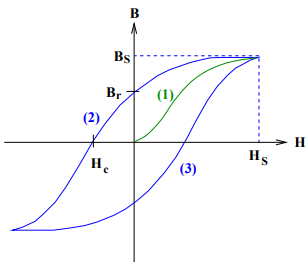
\includegraphics[]{./abbildungen/Hysterese.png}
    \caption[]{Hysteresekurve bei einem veränderlichen äußeren Magnetfeld \cite[]{man:v308}.}
    \label{fig:hysterese}
\end{figure}

\noindent
Wird eine Spule mit einem ferromagnetischen Kern gefüllt, wird der magnetische Fluss der Spule erhöht und kann durch 
\begin{align}
    \symbf{B} = \mu_0 \left(\symbf{H} + \symbf{M}\right)
    \label{eq:Magnetisierung}
\end{align}
quantifiziert werden, wobei $\symbf{M}$ die Magnetisierung beschreibt.
%und für die magnetische Feldstärke $\symbf{H} = \symbf{H}_\text{0} + \symbf{H}_\text{r}$ gilt.
%Dabei werden Randeffekte durch $\symbf{H}_\text{r}$ berücksichtigt.
Bei einer Toroidspule gibt es wie in Abschnitt \ref{sec:toroidspule} geschildert keine Randeffekte.
Außerdem liegt $\mu_\text{r}$ von ferromagnetischen Materialien in einer Größenordnung von $10^2$ bis $10^7$,
sodass sich schließlich 
\begin{align}
    \symbf{B} \simeq \mu_0 \symbf{M} 
    %% Frage: Was bedeutet das, warum ist das wichtig?
\end{align}
ergibt.
